\documentclass[tikz,border=2pt]{standalone}
\renewcommand{\familydefault}{\sfdefault}
\usetikzlibrary{arrows.meta,calc,positioning}
\tikzset{every picture/.style={line width=1pt, >=Stealth},
         hl/.style={fill=black, fill opacity=0.12, text opacity=1}}
\begin{document}
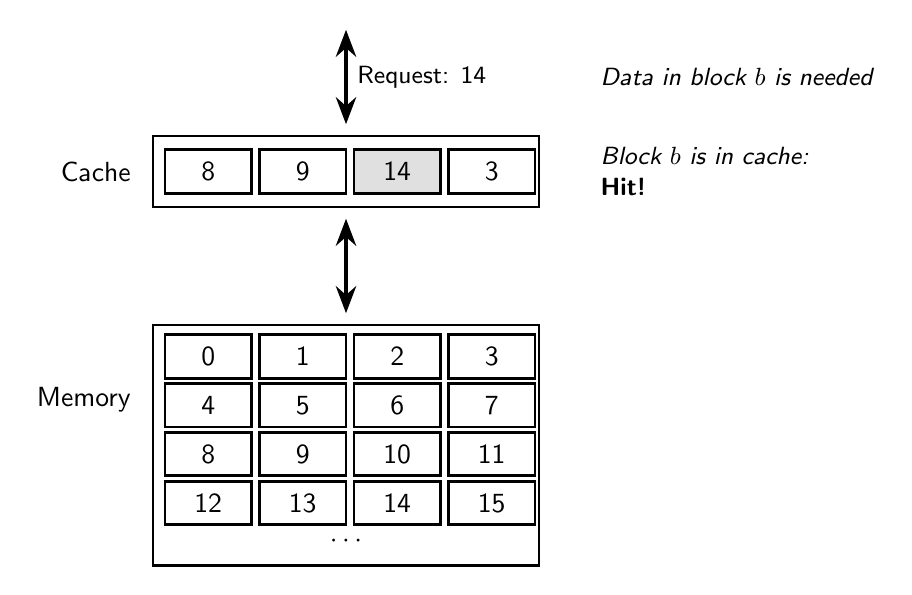
\begin{tikzpicture}[blk/.style={draw, minimum width=1.1cm, minimum height=0.55cm}]
  % The request asks for block 14, which is already in the cache.
  \draw[<->, line width=1.5pt] (2.3, 2.2) -- node[right, font=\small] {Request: 14} (2.3, 1);
  \node[left] at (-0.3, 0.4) {Cache};
  \draw (-0.15, 0.85) rectangle (4.75, -0.05);
  \foreach \b/\s [count=\i from 0] in {8/, 9/, 14/hl, 3/} \node[blk, \s] at (0.55 + 1.2*\i, 0.4) {\b};
  \draw[<->, line width=1.5pt] (2.3, -0.2) -- (2.3, -1.4);
  \node[left] at (-0.3, -2.5) {Memory};
  \draw (-0.15, -1.55) rectangle (4.75, -4.6);
  \foreach \r in {0, ..., 3} \foreach \c in {0, ..., 3} {
    \pgfmathtruncatemacro{\b}{4*\r + \c}
    \node[blk] at (0.55 + 1.2*\c, -1.95 - 0.62*\r) {\b};
  }
  \node at (2.3, -4.3) {$\cdots$};
  \node[anchor=west, align=left, font=\small] at (5.4, 1.6) {\textit{Data in block $b$ is needed}};
  \node[anchor=west, align=left, font=\small] at (5.4, 0.4) {\textit{Block $b$ is in cache:} \\ \textbf{Hit!}};
\end{tikzpicture}
\end{document}
